%\addcontentsline{toc}{chapter}{Development Process}
\chapter{Experiment Methods}

\section{Overview}

The technical outcome of this project was to produce an image analysis pipeline. Broadly speaking the pipeline can be broken into four distinct components. These are feature detection and extraction, dimensionality reduction, quality evaluation, and visualisation.


\begin{figure}
	\label{fig:pipeline-diagram}
	\centering
	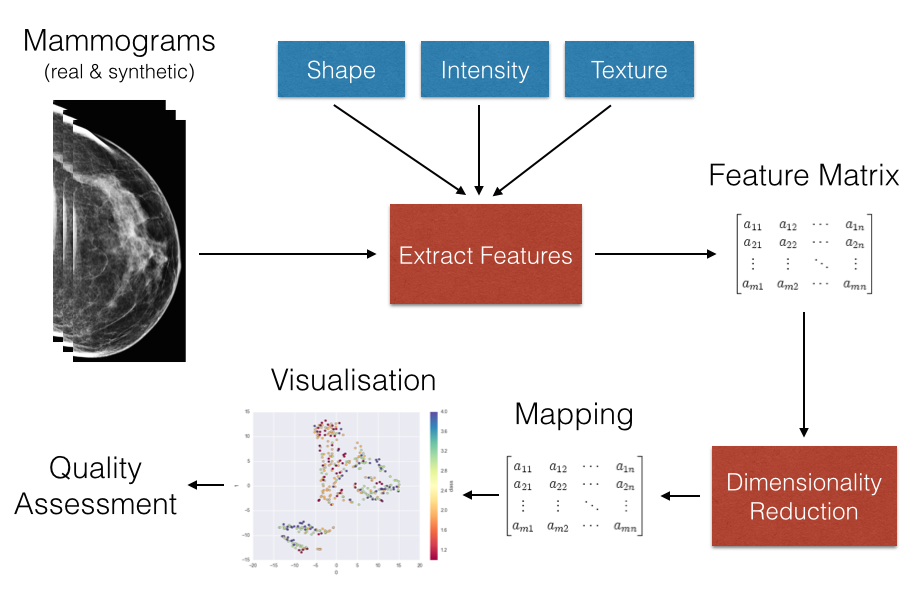
\includegraphics[width=0.8\textwidth]{Images/pipeline-diagram.png}	
	\caption{Conceptual overview of the image analysis pipeline produced as part of this project.}
\end{figure}

\section{Techniques}

\subsection{Preprocessing}
Very little preprocessing of the images has been used in this project. Each of the mammograms used has an accompanying binary mask which is used to remove the background and pectoral muscle (see section \ref{sec:datasets}). The skin around the edge of the breast can cause issues with the blob and line detection due to the intense response during image acquisition. As we are only interested in structure within the parenchyma binary erosion is performed on the breast masks using a disk shaped kernel with a radius of 30 pixels.

\subsection{Features}
\label{sec:features}
In this project we have used three different types of image features to build a feature space from the mammogram datasets. We have used two different types of shape features one to detect blobs and one to detect linear structure. These features intrinsically define a ROI which has some parenchyma pattern of interest. From the ROIs defined by these features we can extract intensity features (based on the image histogram of the ROI) and texture features (in the case of this project GLCM features).

\subsubsection{Blob Features}
The blob detection was achieved by following an approach similar to that described by Chen et al. \cite{chen2013multiscale, chen2013mammographic}. This is a multi-scale approach based on building a Laplacian of Gaussian (LoG) pyramid over ten different scales. 

To obtain a multi-scale view but retain comparative performance (due to the very large size of mammographic images) instead of increasing the size of the kernel the sigma of the Gaussian is fixed to 8.0 and the image is smoothed and downscaled by a factor or $\sqrt{2}$ instead. Once the image has been convolved with the LoG kernel, the resulting image is finally upscaled to full size before peak detection.

Each of the mammographic images in the real dataset come with a set of breast masks which segment the tissue of the breast from the result of the image (such as the pectoral muscle). This helps to ensure that we are detecting the only within the parenchyma but causes issues due to a large edge response produced from the LoG kernel around the edge of the breast. In Chen's thesis this effect was dealt with by means of a "deformable" convolution. The image is convolved with a standard image kernel when the area of the kernel is entirely within the mask area. When the kernel being convolved falls outside of the mask the filter kernel is modified so that it returns zero outside of the mask and the LoG response normalised by the number of nonzero pixels otherwise.

For each scale image produced the local maxima are detected using maximum filter and a conservative threshold. The resulting position of the peak defines the location of the blob detected in the image while the effective sigma of the Gaussian for the scale of the image $\sigma k i$ (where $i$ is the scale and $k$ is the downscale factor equal to $\sqrt{2}$) is the radius of the blob.

This procedure returns a very large number of responses with many overlapping detections. Since we are only interested in blob that best characterises the detected peak, a blob merging strategy is employed to remove redundant blobs. As we are only concerned with blobs that characterise patterns within the parenchyma all blobs whose radius falls outside of the bounds of the image mask are removed. 

Next a thresholding technique is used to remove blobs that fall below a certain level of intensity. The area of the image covered by the blob is categorised into 9 clusters. The average intensity of each cluster is computed and the top 5 clusters are selected. The threshold used is defined to be the average intensity of the top five most intense clusters across all blobs less the standard deviation of those same clusters. 

In Chen's thesis the clustering is performed using the Fuzzy c-means algorithm while in my implementation I have used the k-means algorithm. The result of this is that the algorithm requires more clusters (5 compared to only the top 3 clusters in Chen's thesis) to achieve comparable results.

After these operations the number of blobs detected is significantly reduced but there are still a large number of blobs which significantly overlap one another in high density regions. To achieve a better representation of the distribution of high density tissue in the mammogram blobs are merged according to how they interact one another. The intersections are classified into one of three categories:

\begin{itemize}
	\item External: $d \geq r_A + r_B$
	\item Intersection: $r_A - r_B < d < r_A + r_B$
	\item Internal: $d \leq r_A + r_B$
\end{itemize}

Where $d$ is the distance between the two blobs and the $r_A$ and $r_B$ are the radii of blobs $A$ and $B$. The above definitions assume that $r_A \geq r_B$.

Merging proceeds as follows: if a blob is external then it remains retained. If a blob is internal to a larger (coarser) blob it will be removed. If the blobs intersect one another and they are closely located ($d \leq r_A + \alpha r_B$ for $0 \leq \alpha \leq 1$, assuming $r_A \geq r_B$). In the experiments documented in the report overlap parameter $\alpha$ used was 0.01. 


\subsubsection{Line Features}
Along with shape features based on blobs of high intensity a shape feature based on finding linear structure within a mammogram was used. Linear structure aims to try and characterise the ductal shapes visible in a typical mammogram. For the implementation of this feature we follow the work of Zwiggelaar et al. \cite{zwiggelaar1996finding} and use an orientated bins method to pick out ROIs which may otherwise be missed using just blob features alone.

The orientated bins method proposed in ref. \cite{zwiggelaar1996finding} filters the local neighbourhood of an image by dividing the neighbourhood window into $n$ angular bins with an angular resolution of $\frac{2 \pi}{n}$. The line strength of the local neighbourhood is given by computing the difference between the maximum average intensity of opposing bins and the average intensity of the local neighbourhood as a whole. In the case of a well defined line only one set of opposing bins would give a high response. The orientation of the image is given by the orientation of the maximum bin.

Once the line image for has been generated the results can be enhanced by applying non-maximal suppression \cite{sonka2014image} to the line image to strengthen the detected structure. After suppression the image is once thresholded using a conservative value to remove noise and the image is converted to a binary image. A morphological closing operation is used to improve the connectivity of the line shapes detected from the image. Any points which are within an 8-connectivity of one another are counted as being part of the same structure.

The resulting shape features can be measured by standard first order statistics to produce descriptive features about the blobs and lines detected from the mammogram. Examples of such features are the min, max, and mean size (radius/area) of the shapes detected at each scale.

\subsubsection{Intensity}
The shape features detected using orientated bins and multi-scale blobs define regions of interest across the breast. From these ROIs the patch of the image which is covered by the area or radius of the shape feature can be extracted. The histogram of the intensity values of this image patch provide can provide additional discriminative information about ROI. Descriptive statistics of the ROI such as mean, variance, standard deviation, min, max, upper and lower quartiles can compute from the patch histogram.

\subsubsection{Texture}
As with intensity features, texture features can be extracted from the patches defined by the shapes features as well. In this project we have only used texture features derived from the grey-level co-occurance matrix \cite{haralick1973textural}.

\subsection{Dimensionality Reduction}
In this project the t-SNE as the dimensionality reduction algorithm with which to produce the lower dimensional representations from the higher dimensional feature spaces. The implementation we have used as part of this project is the standard algorithm available through the sci-kit learn library. Before running the dimensionality reduction algorithm the input feature matrix is standardised by removing the mean from each feature and scaling to standard variance.

\subsection{Visualisation}
The visualisation aspects of this project have largely been handled by the inbuilt functionality that available in the matplotlib and pandas Python libraries. However I have also implemented some additional custom visualisation techniques for examining what the images look like for each point in the lower dimensional mapping.

\subsubsection{Visualisation of Images from Mapping}
In order to examine the how images change across the lower dimensional mapping and to try and understand why images are grouped closely together I created a small utility that would read in the mapping of the feature space and display a scatter plot of the mapping. When hovering over each point in the visualisation the image corresponding to that data point is displayed to the right of the scatter plot.

\subsubsection{Median Image Plot}
Similarly to the previous visualisation this visualisation takes a projection of the feature space and creates a two dimensional histogram of the points. From each of the resulting bins the median point in both the $x$ and $y$ directions if found. The image which corresponds to this point is selected to be used as part of the visualisation. Each of the images is stitched together to form a matrix of images in the same shape as the lower dimensional mapping.


\section{Datasets}
\label{sec:datasets}
In this project we are using two different datasets. One consisting of mammograms for taken from a collection of real patients. The other dataset is a collection of artificially generated breast phantoms generously created by the University of Pennsylvania. 

\subsection{Real Data}
The dataset of real mammograms was taken from a private dataset captured using a Hologic full field digital mammography system. The dataset contains images of 90 unique patients each with a craniocaudal and mediolateral oblique view of both the left and right breasts, resulting in 360 total images. Each image in the dataset also has a corresponding binary breast mask. This mask is used to segment the  background and the pectoral muscle from the breast parenchyma.

\subsection{Synthetic Data}
The synthetic breast phantoms were generated by the University of Pennsylvania using the techniques outlined by Bakic et al. \cite{bakic2002mammogram1, bakic2002mammogram2, bakic2003mammogram3}. Their simulation system consists of three major components: a breast tissue model, a compression model, and an acquisition model. Adipose tissue compartments within the breast are modelled using thin shells in areas of primarily adipose tissue and as blobs in areas of predominantly fibroglandular tissue. Ductal lobes are also simulated by the model using a randomly generated tree. 

\section{Implementation}
\label{sec:implementation}
This section provides a brief overview of the implementation details used in the project. All of the methods discussed in the preceding sections were implemented in Python. The technical output of the project is a Python library and command line tool which is used to create the pipeline discussed in the first part of this chapter.

\subsection{Python Package}
The majority of the components used in the project are built upon the top of the scipy stack \cite{jones2014scipy}. Two major additional libraries (which also rely on the scipy stack) which have been used heavily in the project are the scikit image \cite{van2014scikit} and scikit learn \cite{pedregosa2011scikit} projects.

The library created as part of this project forms a complete python package. The package consists of five top level modules and a collection of submodules implementing specific functionality relating to the features detected by the system. The description of each of the modules is as follows:

\begin{itemize}
	\item {\bf reduction}: The reduction module implements functions performing multi-processed feature extraction from a dataset.
	\item {\bf analysis}: The analysis module implements commonly used functions used to analyse the images after feature extraction has been performed. These functions are typically called directly from the python interpreter to in a IPython notebook session.
	\item {\bf plotting}: This module provides a collection of custom, convenience plotting functions that largely depend on the matplotlib library.
	\item {\bf io\_tools}: The io\_tools module implements functions for iterating over directories of images and there corresponding masks as well as image loadings and preprocessing functions.
	\item {\bf utils}: The utils module contains a collection of miscellaneous helper functions used in various places throughout the package.
\end{itemize}

An additional sub-package contains the modules used by the reduction module to perform feature extraction these modules include:

\begin{itemize}
	\item {\bf blobs}: Contains the code implementing blob detection using the approach outlined in section \ref{sec:features}. This also uses an additional private module which provides the code for the graph built as part of the blob merging scheme.
	\item {\bf linear\_structure} Contains the code implementing line feature detection using the approach outlined in section \ref{sec:features}. This also uses a couple of additional private modules within the sub-package which provide the code for non-maximal suppression and the orientated bins feature. 
	\item {\bf texture} Contains the code for computing the GLCM and texture features from ROIs.
	\item {\bf intensity} Contains the code for computing first order statistics from ROIs.
\end{itemize}

The last part of the library is the deformable convolution module. This implements the deformable convolution approach outlined by Chen et al. \cite{chen2013multiscale}. Due to the performance considerations associated with convolution I chose not to write this module directly in Python but to implement it as a C function which is compiled using the Python C API.

\subsection{Command Line Interface}
The command line tools offered by the program are built using the Click library \cite{clickLibrary}. The CLI provides a thin wrapper to the some of the higher level library functions available in the package. The most important commands offered by the CLI are those concerned with image processing to collect features from the images. These functions involve iterating over a folder of images and applying the feature extraction techniques outlined in section  \ref{sec:features}. These operations can take in the order of several hours to complete and so it is useful to have them exposed on the command so they can be run and left until complete. These commands for image reduction also add the ability to automatically dump the output of the reduction to a CSV file named by the user upon completion. 

Other useful commands included in the CLI interface are the ability to run and plot the output of shape feature detection from a single image and the running the t-SNE algorithm on a feature dataset from the command line.




